\chapter{Detection of J0520-2553} \label{app:J0520}

As stated in \cref{sec:results} there was a serendipitous detection of J0520-2553 (see \cref{fig:J0520-2553}), using both the acceleration search and single burst search pipelines in S band. The fluxes were calculated using \cref{eq:radiometer_equation} along with applying an offset from the boresight which is assumed to be Gaussian,  $\exp\left( -\left({4 \ln 2 \cdot \theta^2}\right)/{\text{FWHM}^2} \right)$. Where $\theta$ is the angular separation from the boresight. 

% \begin{equation}
%     \exp\left( -\frac{\theta^2}{2\sigma^2} \right)
% \end{equation}
% TransientX, w = 0.7
\begin{table}[h]
    \centering
    \begin{tabular}{lcc}
        \hline
        Search Method & S/N & \(S_{2000}\) (mJy) \\
        \hline
        PRESTO Folding & 50.2  & 0.05 \\
        PRESTO Single Pulse & 16.6 & 164 \\
        TransientX Single Pulse & 17.2 & 170 \\
        \hline
    \end{tabular}
    \label{tab:J0520_fluxes}
\end{table}


\begin{figure}[h!]
    \centering
    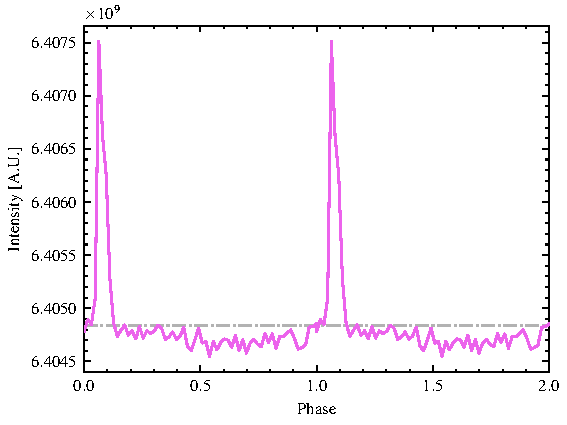
\includegraphics[width=0.7\linewidth]{chapter3/figures/psr-profile-plot.pdf}
    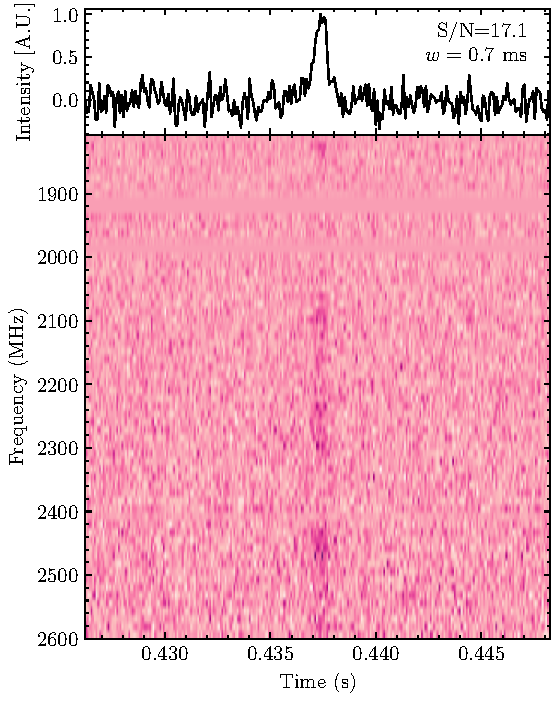
\includegraphics[width=0.7\linewidth]{chapter3/figures/single_burst_dynamic_spectrum.pdf}
    \caption{\textit{Top:} Pulse profile of J0520-2553 obtained from the accelsearch pipeline at a DM of 33.7~\dm. \textit{Bottom:} Single burst pulse also detected at 33.7~\dm~ in S-band.}
    \label{fig:J0520-2553}
\end{figure}